\documentclass[conf]{new-aiaa}
\usepackage[utf8]{inputenc}

\usepackage{graphicx}
\usepackage{subcaption}
\usepackage{amsmath}
\usepackage[version=4]{mhchem}
\usepackage{siunitx}
\usepackage{float}
\usepackage{array}
\usepackage[export]{adjustbox}
\usepackage{longtable, tabularx}
\usepackage{tabulary}
\usepackage{atbegshi,picture}
\usepackage{color, colortbl}
\graphicspath{{./figures/}}
\setlength\LTleft{0pt} 

\title{Particle Filter vs. Extended Kalman Filter Localization for a Mobile Manipulator In ROS2 and Gazebo}

\author{Jacob T. Cassady\footnote{Graduate Student, Robotics and Autonomous Systems, AIAA Member.}}
\affil{Johns Hopkins Whiting School of Engineering, Baltimore, Maryland 21218}

\begin{document}

\maketitle
\begin{abstract}
This abstract will briefly describe the project and the results of the study.
\end{abstract}

\section{Overview}\label{sec:Overview}

A critical precursor to robot path planning is the ability to determine a robot's pose relative to a known environment.
The problem of estimating a robot's pose relative to a known map from proprioceptive measurements and exteroceptive measurements is referred to as localization \cite{thrun2005probabilistic}.
Without a reliable estimate of a robot's state with respect to the world, a robot cannot safely interact with its surroundings.
This paper presents a study comparing algorithms for performing localization of a differential drive mobile manipulator with a two-dimensional (2-D) LiDAR and an odometer.
Each algorithm approximates a probability distribution for the pose, called the \textit{belief}.

To facilitate the development of the algorithms, this study utilizes the Robotic Operating System 2 (ROS2) \cite{macenski2022ros2}.
ROS2 is a middleware framework that is built on top of the Data Distribution Service (DDS) protocol \cite{pardo2003omg} to support distributed architectures.
Within the ecosystem, independent processes are referred to as ``nodes''.
Nodes communicate with one another by publishing and subscribing to shared message queues known as ``topics.''
The distributed architecture enables asynchronous processing of sensor data and commands.

Additionally, this study will make use of the Gazebo simulation environment, which provides a high fidelity physics engine and sensor simulation plugins.
The experiments will take place in a simulated factory world populated with obstacles and goal points for navigation.
Figure \ref{fig:gazebo_sim_2d} illustrates the factory layout, goal points, and the initial position of the robot in 2-D.
Figure \ref{fig:gazebo_sim_3d} provides a screenshot of the factory at runtime in three dimensions (3-D).

\begin{figure}[!htbp]
    \centering
    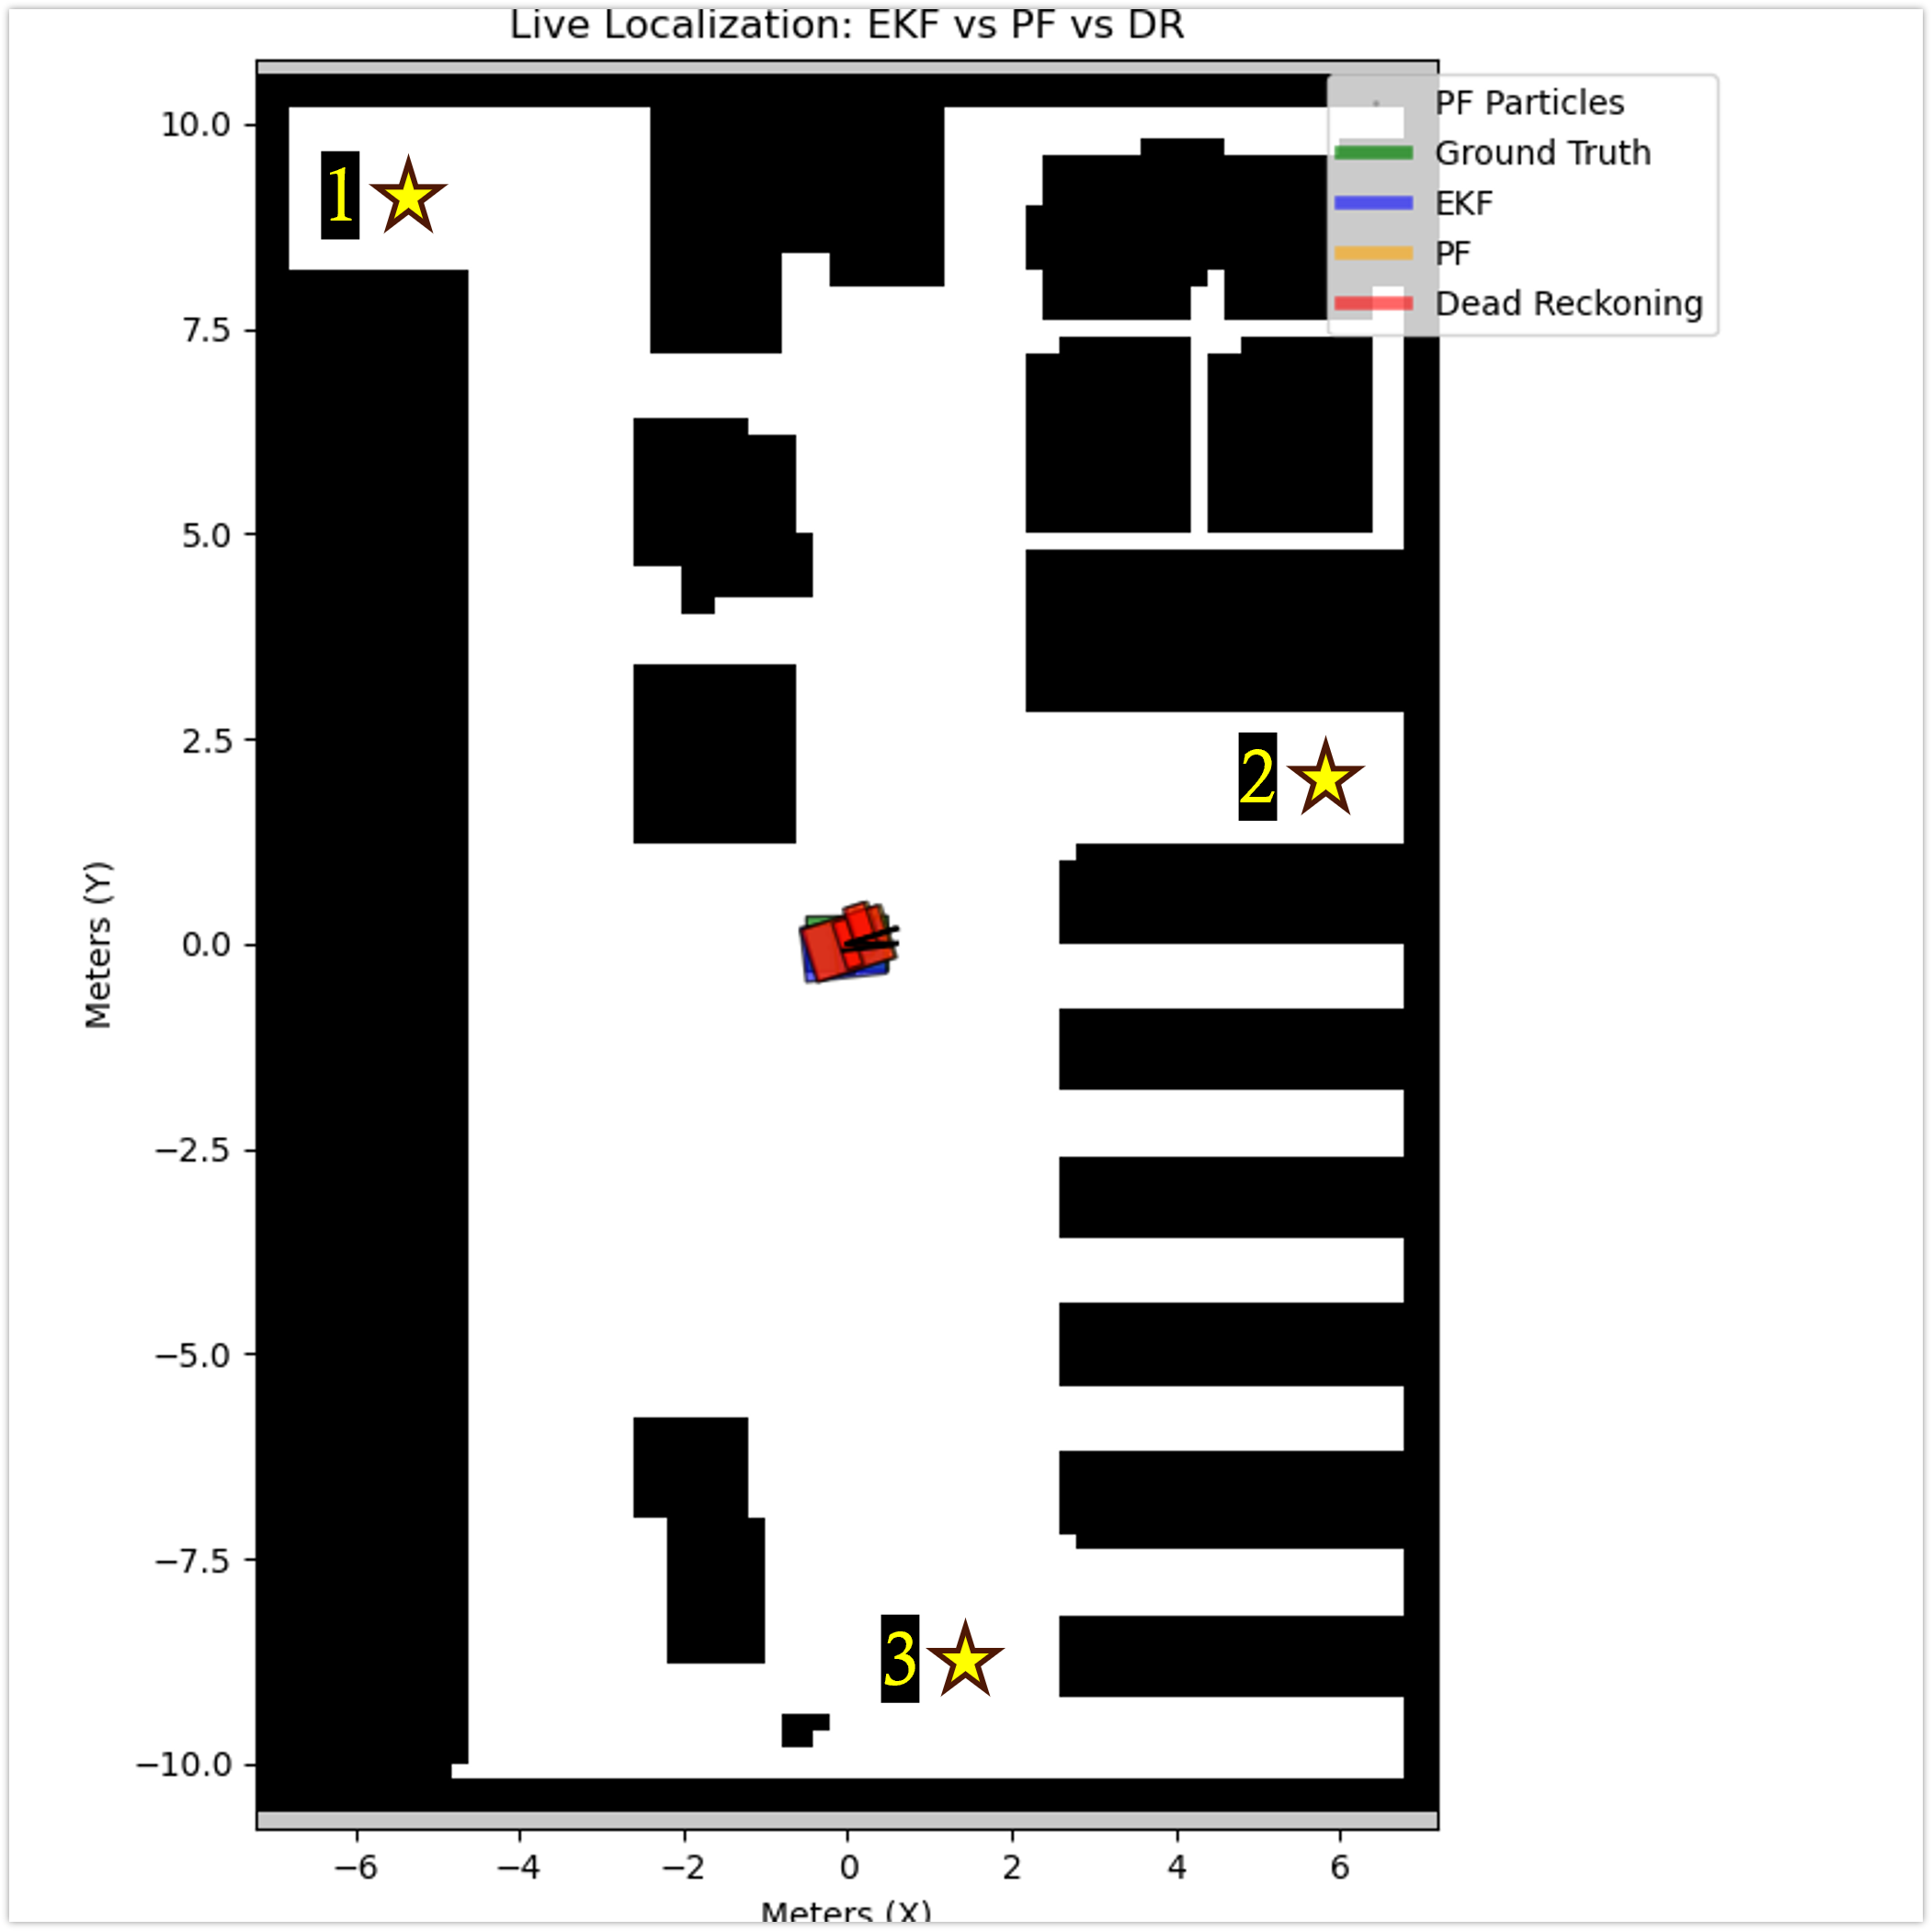
\includegraphics[width=0.6\textwidth]{figures/Devol_Localization_Viz_labeled.png}
    \caption{2-D Rendering of the factory floor, obstacles, and designated goal points.}
    \label{fig:gazebo_sim_2d}
\end{figure}

\begin{figure}[!htbp]
    \centering
    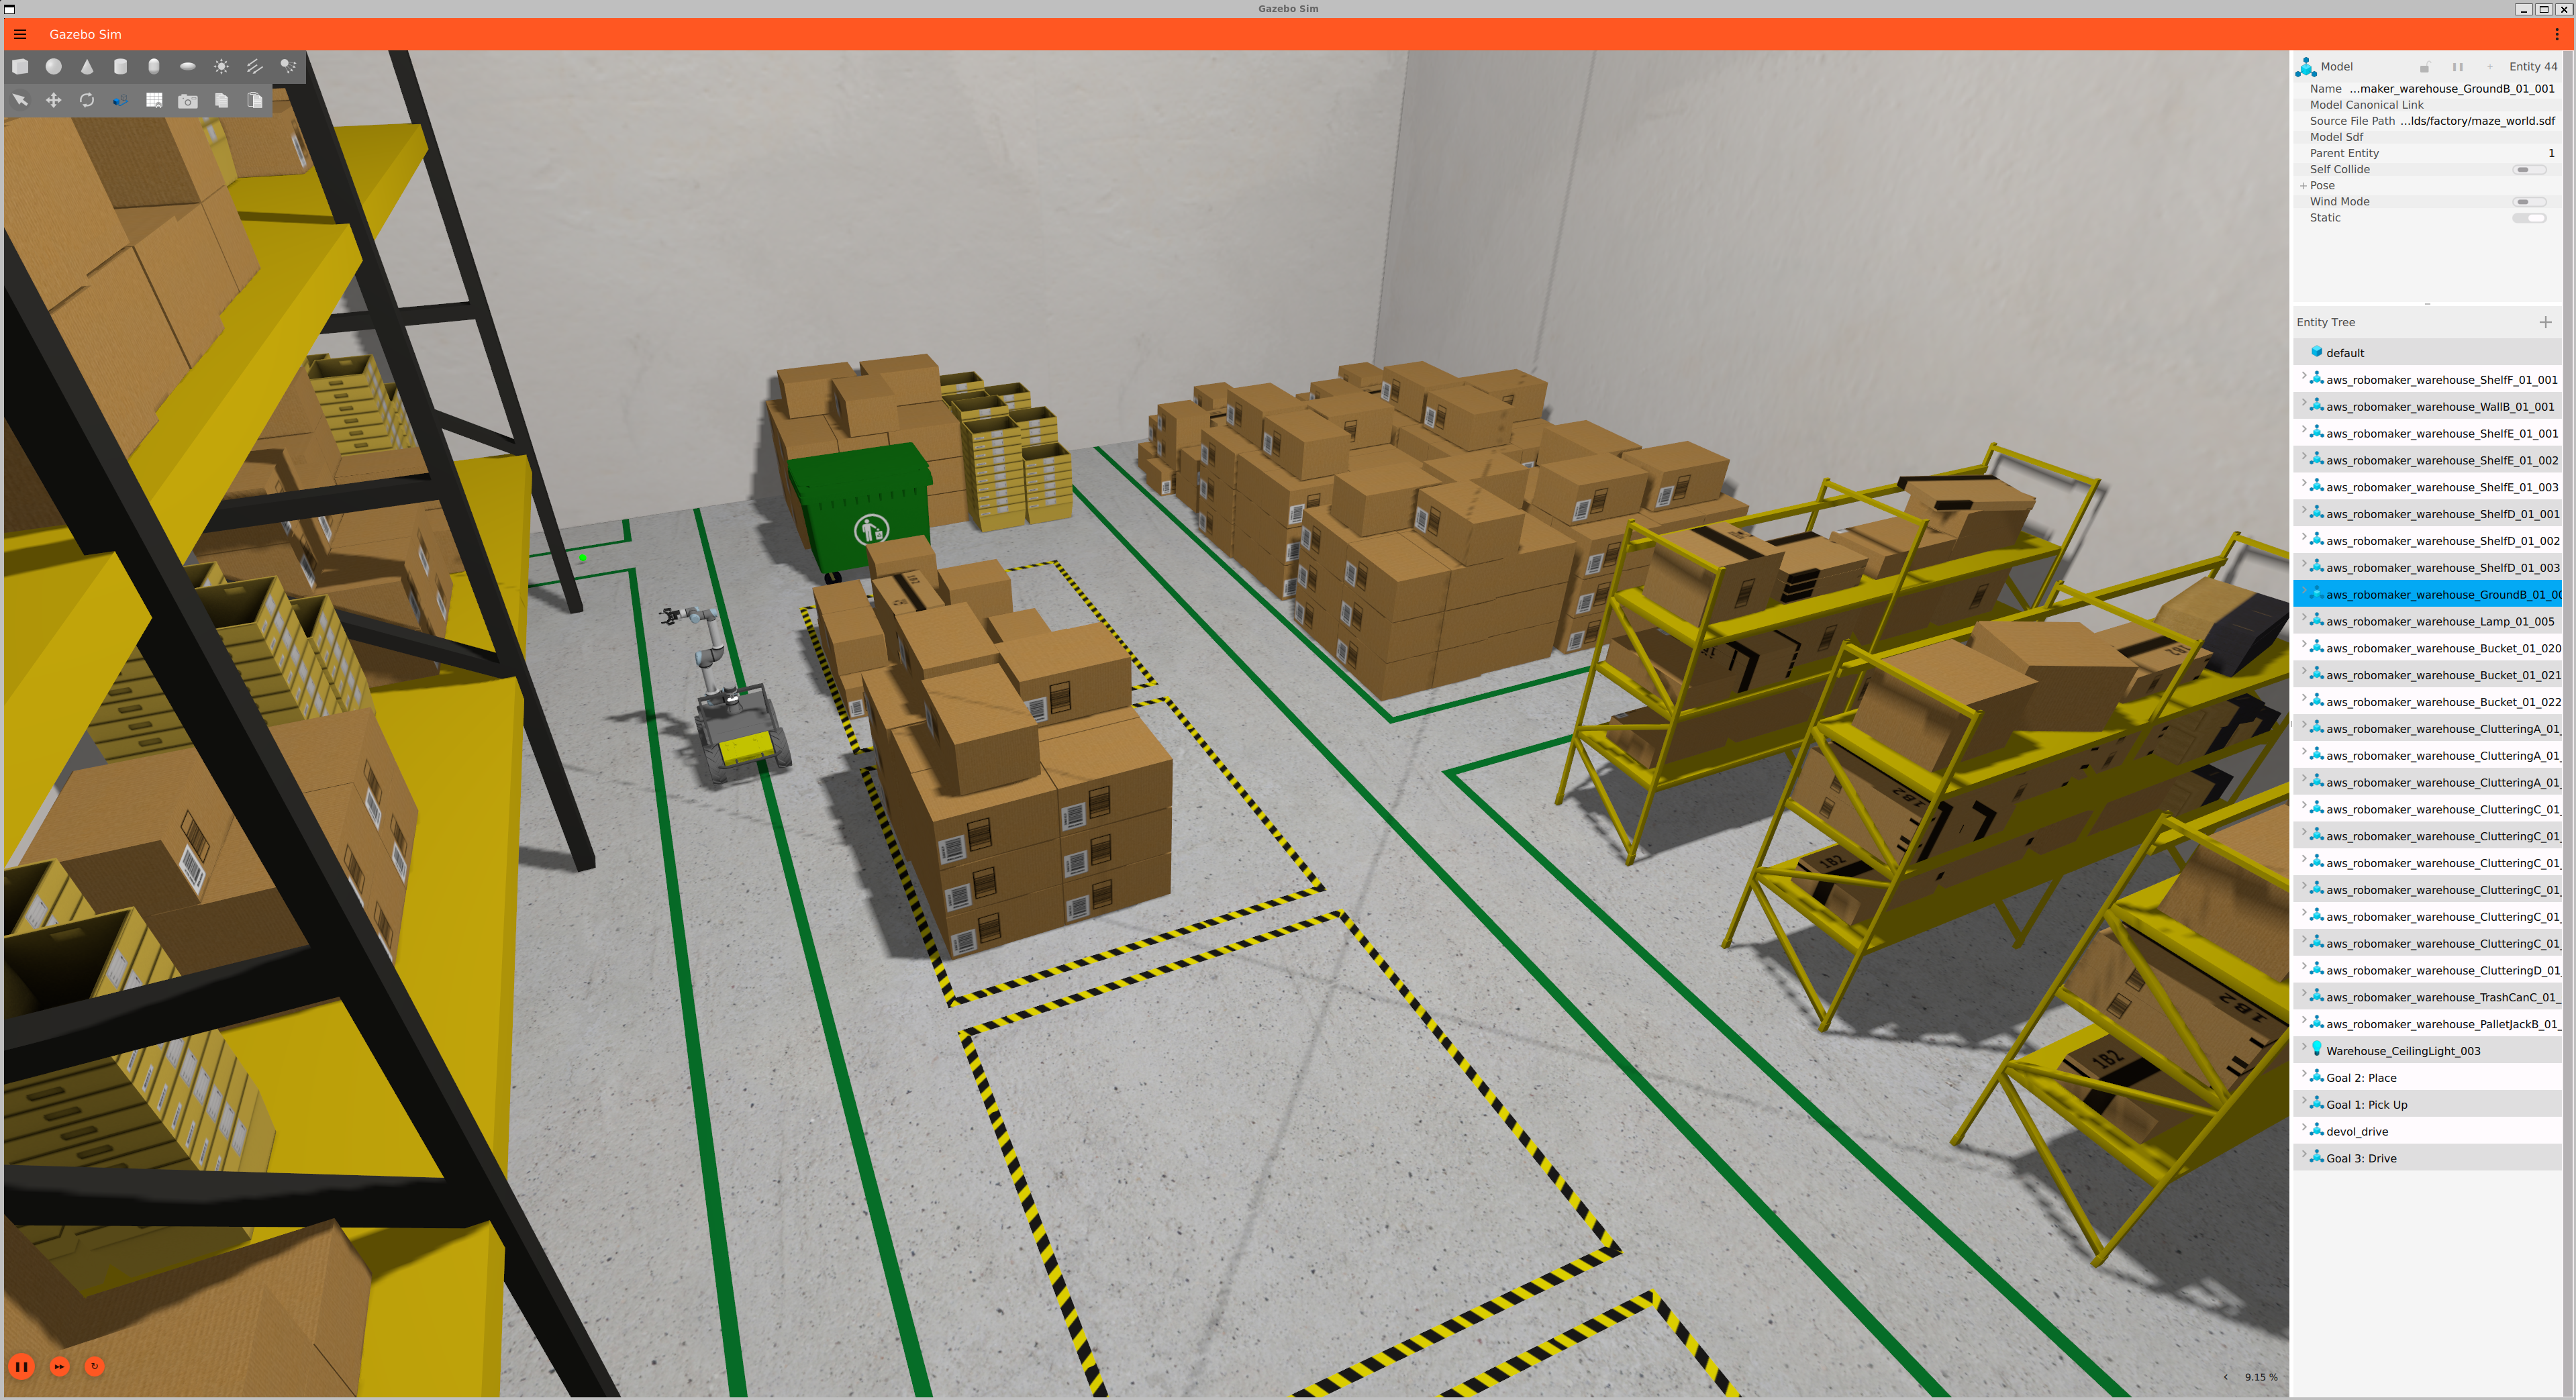
\includegraphics[width=\textwidth]{figures/gazebo_screenshot.png}
    \caption{Gazebo factory 3-D simulation.}
    \label{fig:gazebo_sim_3d}
\end{figure}

The robot models used in Gazebo and ROS2 are defined using Unified Robot Description Format (URDF).
This study will use the mobile manipulator model illustrated in Figure \ref{fig:devol_robot_model}.
It consists of a Husky A200 differential drive mobile platform with a mounted $270^\circ$ 2-D LiDAR and a manipulator.
The manipulator comprises a Universal Robots UR5e collaborative robot arm and a Robotiq 2F-85 end effector.
Additionally, the model makes use of Gazebo's plugins for wheel slip, LiDAR, and odometry.

\begin{figure}[!htbp]
    \centering
    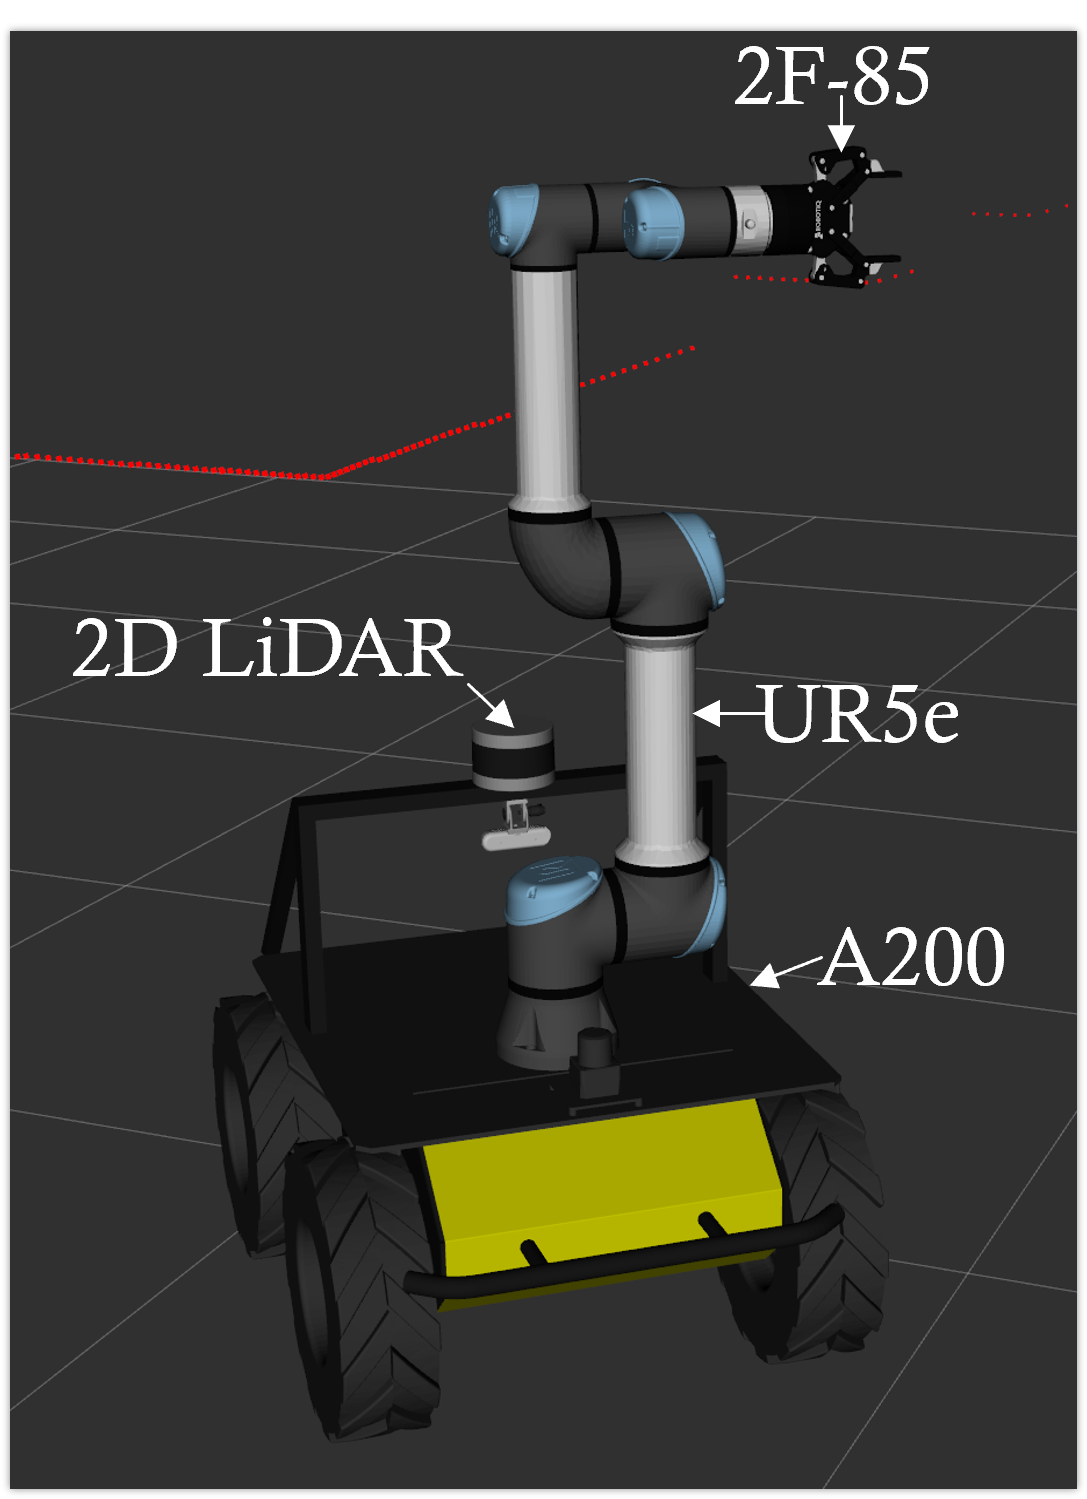
\includegraphics[width=.25\textwidth]{figures/devol_robot_model.png}
    \caption{Test robot model.}
    \label{fig:devol_robot_model}
\end{figure}

The primary objective of this study is to evaluate and compare the performance of different localization algorithms when deployed on a mobile manipulator in a factory setting. 
Specifically, this work investigates the trade-offs between Particle Filter and Extended Kalman Filter approaches. 
By analyzing localization accuracy, computational efficiency, and robustness to sensor noise, this study aims to provide practical insights into selecting the appropriate state estimation strategy for autonomous mobile manipulation.

\section{Problem Statement}\label{sec:Problem-Statement}
In mobile robotics, the planning environment is often projected onto a two dimensional plane.
Let the pose of the robot at time $t$ be defined by the state vector $\mathbf{x}_t = [x_t, y_t, \theta_t]^T$, where $x_t$ and $y_t$ represent the planar coordinates and $\theta_t$ represents the heading. As the robot moves, its true state transitions according to a non-linear motion model:

\begin{equation}
    \mathbf{x}_t = f(\mathbf{x}_{t-1}, \mathbf{u}_t) + \mathbf{w}_t
\end{equation}
where $\mathbf{u}_t$ is the control input (such as wheel velocities) and $\mathbf{w}_t$ represents process noise caused by factors like wheel slip or mechanical imperfections. 

To correct the drift induced by the process noise, the robot relies on exteroceptive sensors, modeled as:
\begin{equation}
    \mathbf{z}_t = h(\mathbf{x}_t) + \mathbf{v}_t
\end{equation}
where $\mathbf{z}_t$ is the sensor measurement (such as a LiDAR scan) and $\mathbf{v}_t$ represents the measurement noise. 
The core problem of localization is to estimate the belief state, or the probability density function $p(\mathbf{x}_t \mid \mathbf{z}_{1:t}, \mathbf{u}_{1:t})$, given all past controls and measurements.

While tracking a robot's pose under normal operating conditions is well understood, catastrophic localization failures remain a significant challenge. 
The most extreme form of this failure is known as the ``kidnapped robot problem'' \cite{DBLP:journals/corr/abs-1106-0222}. 
This occurs when a robot is teleported to a different location without its odometry registering the movement, completely invalidating its current belief state.

In the real world, this could happen if a robot loses power and is re-powered at a different position or if the robot being tracked loses connection with a tracking hub and then reconnects at a different time.
To recover from a kidnapping event, a localization algorithm must be capable of abandoning its incorrect localized belief and search the map to find its new true pose.

Various algorithms exist to solve the localization problem.
The three algorithms selected for this study have different levels of robustness for kidnapping as well as different expected accuracies and computational costs.

The first algorithm, \textbf{Dead Reckoning}, is the most basic form of state estimation.
It relies only on integrating the control inputs $\mathbf{u}_t$ over time to estimate the current pose \cite{ros2_control_mobile_robot_kinematics}.
Because Dead Reckoning lacks a measurement update step, process noise accumulates with time, making the predicted pose stray from truth with time.

The second algorithm, \textbf{Extended Kalman Filter (EKF)} tackles the non-linear motion and measurement models by linearizing them via Taylor series expansion and computing the Jacobians of $f$ and $h$ from the kinematic model and sensor models above \cite{thrun2005probabilistic}.
It assumes the belief state is represented by a single Gaussian distribution characterized by a mean vector and a covariance matrix.

The third algorithm, \textbf{Particle Filter (PF)}, is a non-parametric approach that represents the belief state using finite sets of weighted random samples called particles \cite{doucet2000sequential}.
Because the PF does not assume a single Gaussian distribution as the EKF does, the PF can represent complex, multi-modal beliefs.

This study evaluates these algorithms under various factory conditions to test two primary hypotheses. First, it is hypothesized that the Particle Filter will recover localization accuracy following a kidnapping event significantly more reliably than the Extended Kalman Filter. 
This is due to the Particle Filter's ability to maintain multiple pose hypotheses simultaneously. 
Second, it is hypothesized that given a well-defined Gaussian initial pose prior (where the robot's starting location is known), the Extended Kalman Filter will achieve localization accuracy comparable to or better than the Particle Filter while requiring a significantly lower computational cost.

% \section{System Model}\label{sec:System-Model}
% This section details the model that the three algorithms share including the mobile platform and its sensors, the kinematic model and its Jacobians, the odometry noise model, the laser geometry, and the map representations.

% \subsection{Platform and Sensors}
% The simulated mobile platform is a Clearpath Husky A200 which is a four-wheeled skid-steer vehicle.
% The simulated mobile platform utilizes Gazebo's \texttt{DiffDrive} plugin which treats the two left and two right wheels as one wheel per side and computes a body twist from the mean wheel spin rates $\dot{\varphi}_L$ and $\dot{\varphi}_R$ with the standard differential-drive relations \cite{lynch2017modern}.

% \[
% v=\frac{r_w (\dot{\varphi}_R+\dot{\varphi}_L)}{2}, \omega^{\text{odom}}=\frac{r_w (\dot{\varphi}_R-\dot{\varphi}_L)}{B_p}
% \]

% Where the constants $r_w$, the wheel radius, and $B_p$, the wheel separation, are provided to the DiffDrive plugin in the URDF.
% And the calculated values $v$ and $\omega^\text{odom}$ represent the forward speed in (m/s) and the yaw rate respectively.
% These values are packaged by the plugin and reported on the topic \texttt{/odom}.

% The simulated mobile platform also utilizes the 

\section{Study Approach}\label{Study-Approach}

This section details the mathematical formulations and algorithm implementations used in this study. It also outlines the ROS2 data flow, the metrics collected for evaluation, and the experimental design. 

\subsection{ROS2 Design}\label{subsec:Dead-Reckoning}

\begin{figure}[!htbp]
    \centering
    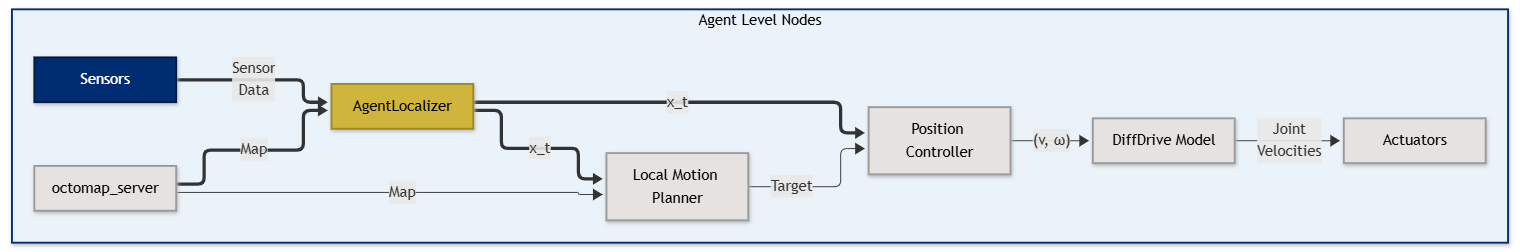
\includegraphics[width=\textwidth]{figures/full_system_diagram.png}
    \caption{Full ROS2 system diagram}
    \label{fig:full_system_diagram}
\end{figure}

\subsection{Dead Reckoning}\label{subsec:Dead-Reckoning}
Dead Reckoning is a classic state estimation algorithm that includes a prediction step using a kinematic model and no update step.
While the robot is physically a differential drive platform, the raw wheel encoders are abstracted upstream by the ROS2 odometry system. 
Thus, the robot's motion is mathematically formulated using the \textbf{Unicycle Kinematic Model} \cite{ros2_control_mobile_robot_kinematics}.

To account for systematic odometry errors that change dynamically during operation such as wheel sliping, this study employs an online self-calibration approach \cite{roy1999online}. 
The state vector is expanded to include a dimensionless yaw rate scale factor $s_t$, making the augmented state $\mathbf{x}_t = [x_t, y_t, \theta_t, s_t]^T$.

Let the raw control input at time $t$ be defined as $\mathbf{u}_t = [v_t, \omega_t]^T$, where $v_t$ is the linear velocity and $\omega_t$ is the raw angular velocity provided by the odometry topic. 
The true angular velocity is estimated as the product of the raw angular velocity and the scale factor $s_{t-1}$. 
Given a time step $\Delta t$, the state estimate is computed using an augmented Unicycle Kinematic Model:

\textbf{Prediction Step:} Let the control input at time $t$ be defined as $\mathbf{u}_t = [v_t, \omega_t]^T$, where $v_t$ is the linear velocity and $\omega_t$ is the angular velocity provided by the odometry topic. Given a time step $\Delta t$, the state estimate is computed as:
\begin{equation} \label{eq:dead_reckoning}
    \begin{bmatrix} x_t \\ y_t \\ \theta_t \end{bmatrix} = 
    \begin{bmatrix} x_{t-1} \\ y_{t-1} \\ \theta_{t-1} \end{bmatrix} +
    \begin{bmatrix} v_t \cos(\theta_{t-1}) \Delta t \\ v_t \sin(\theta_{t-1}) \Delta t \\ \omega_t \Delta t \end{bmatrix}
\end{equation}

To quantify the accumulating uncertainty of this open loop integration, the system also tracks the state covariance $\Sigma_t$. To accurately model the kinematic uncertainty of a differential drive robot, process noise is modeled in the control space rather than the global state space \cite{thrun2005probabilistic}. The uncertainty of the velocity commands is proportional to the commanded velocities themselves, defined by the error coefficients $\alpha_1$ through $\alpha_4$:
\begin{equation}
\sigma_v = \alpha_1 |v_t| + \alpha_2 |\omega_t|
\end{equation}
\begin{equation}
\sigma_\omega = \alpha_3 |v_t| + \alpha_4 |\omega_t|
\end{equation}
These standard deviations form the control noise covariance matrix $M_t$:
\begin{equation}
M_t = \begin{bmatrix} \sigma_v^2 & 0 \\ 0 & \sigma_\omega^2 \end{bmatrix}
\end{equation}

To map this control noise into the global state space, we compute the Jacobian of the motion model with respect to the control inputs, denoted as $V_t$:
\begin{equation}
V_t = 
\begin{bmatrix} 
\cos(\theta_{t-1}) \Delta t & 0 \\ 
\sin(\theta_{t-1}) \Delta t & 0 \\ 
0 & \Delta t 
\end{bmatrix}
\end{equation}
The mapped process noise matrix $R_t$ is then calculated by projecting the control covariance through this Jacobian:
\begin{equation}
R_t = V_t M_t V_t^T
\end{equation}

Finally, the predicted covariance $\Sigma_t$ is updated using the state Jacobian $G_t$ and the mapped process noise $R_t$:
\begin{equation} \label{eq:dr_cov}
\Sigma_t = G_t \Sigma_{t-1} G_t^T + R_t
\end{equation}
where $G_t$ is the Jacobian of the motion model with respect to the state $\mathbf{x}$. For the unicycle model, this Jacobian is analytically derived as:
\begin{equation}
    G_t = 
    \begin{bmatrix} 
    1 & 0 & -v_t \sin(\theta_{t-1}) \Delta t \\ 
    0 & 1 & v_t \cos(\theta_{t-1}) \Delta t \\ 
    0 & 0 & 1 
    \end{bmatrix}
\end{equation}
Because Dead Reckoning lacks a measurement update step, this covariance grows unbounded over time, visually representing the drift of the open loop system.

\subsection{Extended Kalman Filter (EKF)}\label{subsec:EKF}
The EKF fuses the Dead Reckoning prediction with the ICP measurement update. Because the system is non-linear, the EKF linearizes the measurement models using Jacobians \cite{leonard1991mobile}. 

\textbf{Prediction Step:} The EKF prediction step is identical to the probabilistic Dead Reckoning process described in Section \ref{subsec:Dead-Reckoning}. This yields the predicted state $\mathbf{\bar{x}}_t$ (via Equation \ref{eq:dead_reckoning}) and the predicted covariance $\bar{\Sigma}_t$ (via Equation \ref{eq:dr_cov}).

\textbf{Update Step:} When an ICP measurement $\mathbf{z}_t$ is received, the measurement residual (innovation) $\mathbf{y}_t$ and the innovation covariance $S_t$ are computed:
\begin{equation}
    \mathbf{y}_t = \mathbf{z}_t - \mathbf{\bar{x}}_t
\end{equation}
\begin{equation}
    S_t = H_t \bar{\Sigma}_t H_t^T + Q_t
\end{equation}
where $H_t$ is the Jacobian of the measurement model (which is the identity matrix $I$ in this direct observation setup), and $Q_t$ is the measurement noise covariance matrix.

The Kalman Gain $K_t$ is then calculated to weight the measurement against the prediction:
\begin{equation}
    K_t = \bar{\Sigma}_t H_t^T S_t^{-1}
\end{equation}
Finally, the state and covariance are updated:
\begin{equation}
    \mathbf{x}_t = \mathbf{\bar{x}}_t + K_t \mathbf{y}_t
\end{equation}
\begin{equation}
    \Sigma_t = (I - K_t H_t) \bar{\Sigma}_t
\end{equation}

\subsubsection{Scan Matching via ICP and SVD}\label{subsec:ICP}
To provide measurement updates to the Extended Kalman Filter, this study utilizes 2-D LiDAR scan matching against a known map. The Iterative Closest Point (ICP) algorithm is employed to align the current LiDAR scan with a reference map \cite{besl1992method}. 

Because the correspondence between the LiDAR points and the map obstacles is unknown, the algorithm proceeds iteratively. At each iteration, the LiDAR points are projected into the global frame using the current pose estimate. A KD-Tree is utilized to efficiently find the nearest neighbor in the reference map for each projected LiDAR point. To prevent geometric distortion, matches that exceed a maximum distance threshold are rejected as outliers.

Given this resulting set of $N$ inlier source points from the LiDAR scan $P = \{\mathbf{p}_1, \mathbf{p}_2, ..., \mathbf{p}_N\}$ and the corresponding nearest-neighbor target points from the map $Q = \{\mathbf{q}_1, \mathbf{q}_2, ..., \mathbf{q}_N\}$, the goal is to find the optimal rotation matrix $R$ and translation vector $\mathbf{t}$ that minimizes the sum of squared errors between the point sets. This is solved analytically using Singular Value Decomposition (SVD) \cite{arun1987least}.

First, the centroids of both point clouds are computed:
\begin{equation}
\mathbf{\bar{p}} = \frac{1}{N} \sum_{i=1}^N \mathbf{p}_i, \quad \mathbf{\bar{q}} = \frac{1}{N} \sum_{i=1}^N \mathbf{q}_i
\end{equation}
The point clouds are then centered by subtracting their respective centroids:
\begin{equation}
\mathbf{p}'_i = \mathbf{p}_i - \mathbf{\bar{p}}, \quad \mathbf{q}'_i = \mathbf{q}_i - \mathbf{\bar{q}}
\end{equation}
Next, the cross-covariance matrix $H$ is computed:
\begin{equation}
H = \sum_{i=1}^N \mathbf{p}'_i (\mathbf{q}'_i)^T
\end{equation}
SVD is then applied to the matrix $H$ such that $H = U \Sigma V^T$. The optimal rotation matrix $R$ is recovered as:
\begin{equation} \label{eq:svd_rotation}
R = V U^T
\end{equation}
To prevent reflection matrices (where the determinant of $R$ is $-1$), a correction is applied by multiplying the last column of $V$ by $-1$ if necessary. Finally, the translation vector $\mathbf{t}$ is computed:
\begin{equation} \label{eq:svd_translation}
\mathbf{t} = \mathbf{\bar{q}} - R \mathbf{\bar{p}}
\end{equation}
The resulting rigid transformation $[R \mid \mathbf{t}]$ yields the measurement vector $\mathbf{z}_t = [x_{obs}, y_{obs}, \theta_{obs}]^T$ which is fed into the EKF.

The Particle Filter, implemented as Monte Carlo Localization (MCL), represents the belief state using a set of $M$ particles: $\mathcal{X}_t = \{ \mathbf{x}_t^{[m]}, w_t^{[m]} \}_{m=1}^M$, where $\mathbf{x}_t^{[m]}$ is a pose hypothesis and $w_t^{[m]}$ is its corresponding importance weight \cite{fox1999monte}. The MCL algorithm proceeds in three standard phases.

\textbf{Prediction (Sampling):} For each particle $m$, a new pose hypothesis is sampled from the probabilistic motion model:
\begin{equation}
\mathbf{x}_t^{[m]} \sim p(\mathbf{x}_t \mid \mathbf{x}_{t-1}^{[m]}, \mathbf{u}_t)
\end{equation}
This is achieved by applying the unicycle kinematics and injecting the exact same proportional control noise defined in Section \ref{subsec:Dead-Reckoning}. Because the particles represent individual state hypotheses, this control noise is sampled stochastically and added to the velocity commands before being passed through the forward kinematic model.

\textbf{Update (Weighting):} The weight of each particle is updated using a Likelihood Field sensor model \cite{thrun2005probabilistic}. Rather than extracting a direct pose estimate from the scan like the EKF, the PF evaluates the raw LiDAR ranges against a pre-computed distance transform map. For a given particle pose hypothesis, each LiDAR endpoint $k$ is projected into the global map to find its Euclidean distance $d_k$ to the nearest obstacle. Assuming zero-mean Gaussian sensor noise with standard deviation $\sigma_{hit}$, the likelihood of a single beam is:
\begin{equation}
p(z_t^k \mid \mathbf{x}_t^{[m]}) \propto \exp \left( -\frac{d_k^2}{2\sigma_{hit}^2} \right)
\end{equation}
The total weight for particle $m$ is proportional to the product of the likelihoods of all valid beams. To prevent numerical underflow in floating-point operations, this is computed in log-space using the log-sum-exp trick:
\begin{equation}
w_t^{[m]} = \eta \exp \left( \sum_{k} \log p(z_t^k \mid \mathbf{x}_t^{[m]}) \right)
\end{equation}
where $\eta$ is a normalization constant ensuring that $\sum_{m=1}^M w_t^{[m]} = 1$.

\textbf{Resampling:} To prevent particle deprivation, where a majority of the computational effort is spent updating particles with near zero weights, low variance resampling is applied. 
A new set of $M$ particles is drawn from the current set with replacement, where the probability of drawing particle $m$ is proportional to its weight $w_t^{[m]}$. 
This focuses the distribution on the most probable regions of the state space.

This section will focus on the algorithm implementations, ROS2 data flow, metrics, and experiment design.
It will detail the localization algorithms for dead reckoning \cite{ros2_control_mobile_robot_kinematics}, extended kalman filter (EKF) \cite{leonard1991mobile}, and particle filter (PF) \cite{doucet2000sequential}.
It will describe scan matching, including the iterative closest point (ICP) algorithm \cite{besl1992method}, as well as, details on the SVD-based rigid transformation \cite{arun1987least}.
Furthermore, this section will detail the design of Monte Carlo Localization (MCL) algorithm for the PF \cite{fox1999monte}.
If time permits, this section will describe a hybrid algorithm in which the PF detects potential kidnapping events and supports EKF recovery by providing a pose estimate and an uncertainty estimate derived from the particle distribution.

The study approach section will continue with ROS2 node graph and data flow focusing on the inputs and outputs for the localization algorithms.
It will detail where data is being produced, where noise is being injected, and the plans for storing the data for analysis.
Next, this section will detail the metrics that will be collected at each time step including position error, heading error, and compute cost.
Finally, this section will detail the experimental design for test cases including a uniform prior, mid-run kidnapping, the sensitivity analyses on varying particle count, injected odometry noise, and injected LiDAR noise.

\section{Results}\label{Results}
This section will present the results of the study.
It will graph the localization error over time, position RMSE in meters, heading RMSE in radians, and compute cost in seconds for the three algorithms (or four if I finish the hybrid algorithm) with 95\% confidence intervals.
A second set of graphs will be made for results in the kidnapping studies.
Additionally, this section will provide the findings for the sensitivity analyses described in the study approach including varying particle count, injected odometry noise, and LiDAR noise.

\section{Conclusion}\label{Conclusion}
The final section will restate the problem statement.
It will briefly overview the study approach and remark on the results and their implications.
This section will include notes on limitations of the study and the conclusion will end with a discussion on future work with a focus on what would need to change to apply these algorithms to a sloped map.

\bibliography{ref}

\end{document}